\section{Optimisation à l'aide de structure arborescente}
%++++++++++++++++++++++++++++++++++++++++++++++++
\subsection{Implémentation de Bounding Volume Hierarchy (BVH)}
%------------------------------------------------
\begin{frame}[fragile]
\frametitle{Principe de BVH\esp}

\begin{tabular}{p{.5\textwidth}p{.5\textwidth}}
\flushleft  
Division des objets dans un arbre selon leur position 
\medskip 

Chaque noeud contient :
\begin{itemize}
    \item Une sphère englobant les objets 
    \item La liste des objets contenus dans ce noeud
    \item Les deux noeuds fils
\end{itemize}

    & \flushright 
        \begin{figure}[H]
            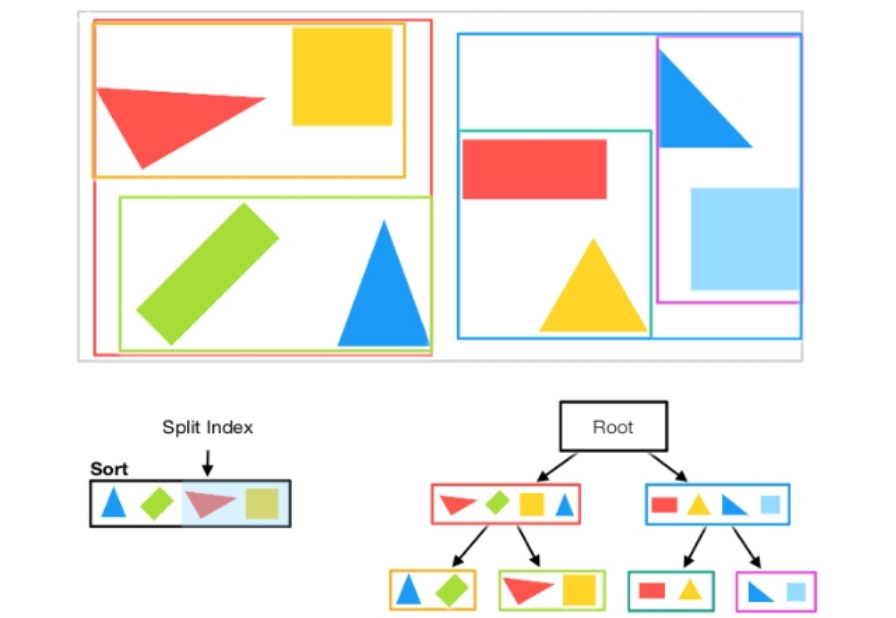
\includegraphics[width=6cm]{ImagesElio/BVH.png}
        \end{figure}
\end{tabular}

\end{frame}


%------------------------------------------------
\begin{frame}[fragile]
\frametitle{Parcours de BVH\esp}
\tiny 
\begin{algorithm}[H]
    \caption{\textsf{TraverseBVH}}
    \Input{Noeud racine $N=(S,l,g,d)$, position $p$}
    \Output{Plus courte distance de $p$ aux objets de la scène}
    \BlankLine
    Initialiser $d1$ à la distance entre $p$ et la sphère englobante gauche\;

    Initialiser $d2$ à la distance entre $p$ et la sphère englobante droite\;

    %{\footnotesize\tcc*{~La source est la racine de l’arborescence }}
    $dist \gets +\infty$\;
    %{\footnotesize\tcc*{~La racine est le premier sommet à traiter }}
    \If{$N$ est une feuille}{
        $dist \gets \min_i{(dist(p,l[i]))}$\;
    }
    \ElseIf{$d1 < d2$}{
        $dist \gets$ TraverseBVH($g, p$)\;
        \If{$d2 < dist$}{ 
            $dist \gets$ min($dist$, TraverseBVH($d,p$))\;
        }
    }	
    \Else{
        $dist \gets$ TraverseBVH($d, p$)\;
        \If{$d1 < dist$}{ 
            $dist \gets$ min($dist$, TraverseBVH($g,p$))\;
        }
    }
\Return{$dist$}
\end{algorithm}
\end{frame}


%------------------------------------------------
\begin{frame}[fragile]
\frametitle{Utilité et mise en pratique}

Implémentation en C de la structure d'objet :
\begin{lstlisting}[c]
Objet :
  Type    // cube, sphere...
  Centre          
  Rayon   // aide au calcul de sphere englobante
  Couleur
  Parametres  // sous forme de void*
\end{lstlisting}
\medskip

La structure de BVH :
\begin{itemize}
    \item est construite une seule fois pour des objets fixes.
    \item réduit les calculs pour une scène comportant beaucoup d'objets
\end{itemize}

\end{frame}


%++++++++++++++++++++++++++++++++++++++++++++++++
\subsection{Manipulation d'objets en mouvements}
%------------------------------------------------
\begin{frame}[fragile]
\frametitle{Gestion des objets en mouvement}
Construction de 2 arbres : 
\begin{itemize}
    \item Un BVH contenant les objets fixes calculé au début de la boucle
    \item Un BVH contenant les objets en mouvement recalculé pour chaque image
\end{itemize}
\\[1cm]

\end{frame}


%++++++++++++++++++++++++++++++++++++++++++++++++
\subsection{Bilan, gain de temps}
%------------------------------------------------
\begin{frame}[fragile]
\frametitle{Bilan et gains}
\label{derniere_slide_effective}
\end{frame}

Temps de génération et de libération de l'arbre négligeables (0,04s pour la scène 1)
\medskip 

\begin{tabular}{p{.5\textwidth}p{.5\textwidth}}
    \flushleft  
    Scène test 1 :  
    \medskip 
    
    \begin{figure}
        \includegraphics[width=5cm]{ImagesElio/Simpson.jpg}
    \end{figure}
    \medskip

    6500 triangles
    \smallskip

    6 threads, écran de 960x540 :

    \hspace{1cm}
    7min
    
        & \flushright 
        Scène test 2 : 
        \medskip 

            \begin{figure}[H]
                \includegraphics[width=5cm]{ImagesElio/Plage.jpg}
            \end{figure}
            \medskip 

            3000 triangles 
            \medskip 

            6 threads, écran de 960x540 :

            \hspace{1cm}
            40s
    \end{tabular}


%------------------------------------------------
\begin{frame}[fragile]
\frametitle{Slide bonus qui ne compte pas}
\end{frame}


%------------------------------------------------
\begin{frame}[fragile]
\frametitle{Encore une slide bonus qui ne compte pas}
\end{frame}
\addtocounter{framenumber}{-2} 


